\documentclass{../ficheTDTP}
\usepackage{hyperref}
\usepackage{tikz}
\usetikzlibrary{positioning,shapes,shadows,arrows,fit}

\title{Projet Nénuphars}
\def \pname{nenuphars}


\begin{document}%

\maketitle

\begin{figure}[h]
\vspace{-5mm}
	\begin{center}
            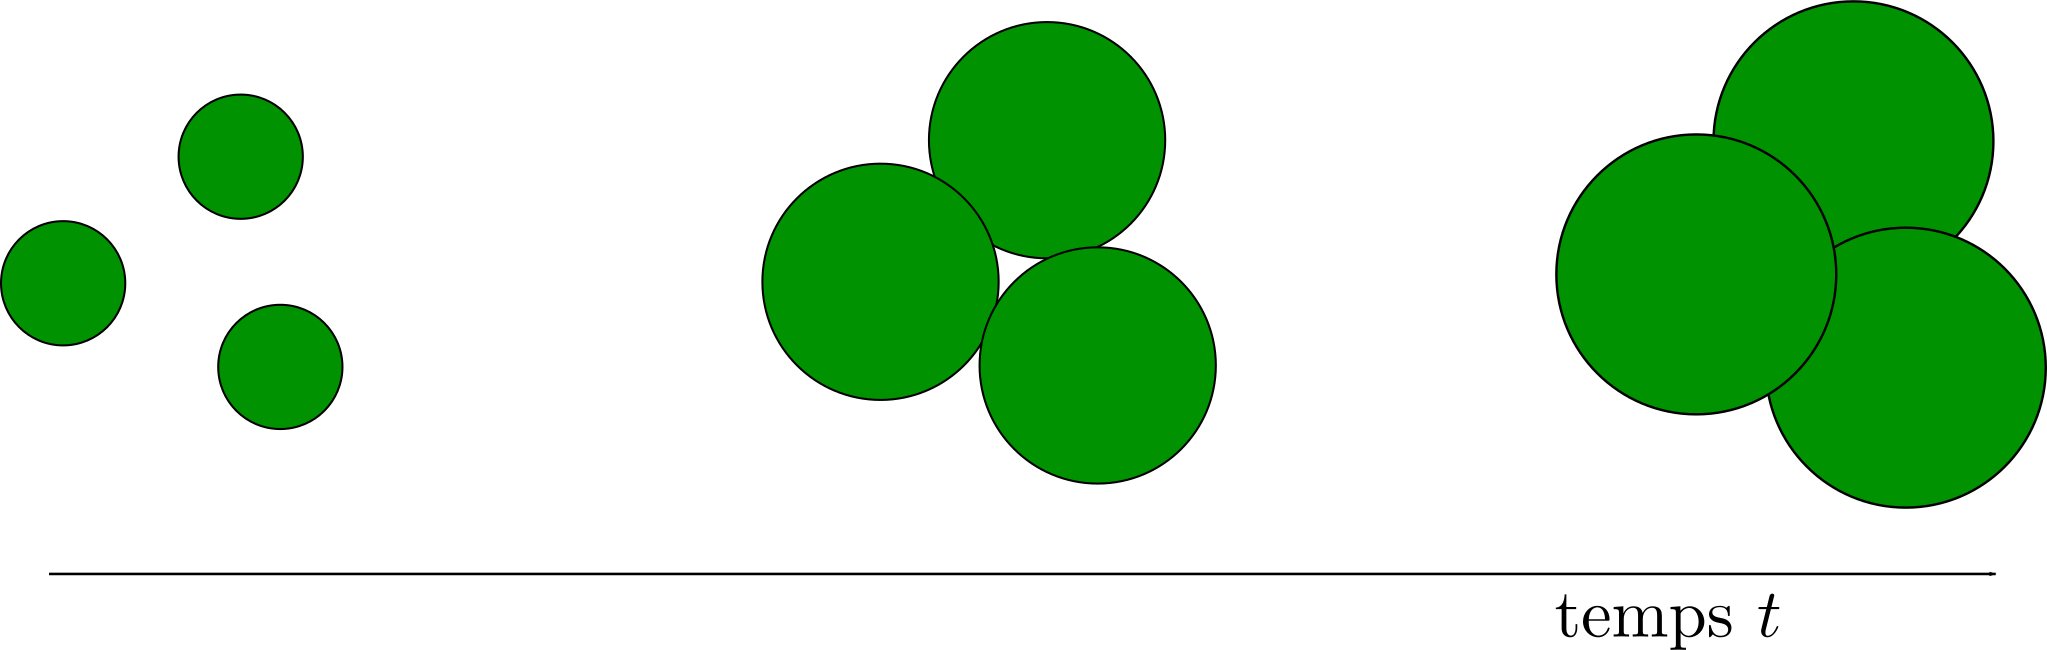
\includegraphics[width=4cm]{nenuphar.jpg}
        \end{center}

\end{figure}

\section*{Introduction}

	Le but de ce projet est d'étudier et de simuler la croissance de nénuphars sur un lac et d'étudier les aspect géométriques de leur configuration. Ce type de problème a de nombreuses applications non seulement si l'on cherche à étudier les néphuphars mais aussi pour toutes les questions de couverture du territoire, par exemple couverture réseau. \\

\textbf{Mots-clés : géométrie, simulation.}

\medskip

Le principe du projet est d'étudier une question mathématique complexe de façon autonome et originale en utilisant l'outil informatique. \textbf{L'ensemble du projet est à faire par groupe de 3 étudiants.} Le projet est divisé en 2 sections : théorique et pratique. La première partie est \textbf{obligatoire}, la seconde partie correspond à des \textbf{pistes de travail}.

\subsection*{Rendu du projet}\strut

Vous devrez rendre:

\begin{itemize}

\item un \textbf{rapport de mi-projet} répondant aux questions de la section 1;

\item un \textbf{exposé} en fin de projet présentant votre travail et vos résultats sur la section 2.
\end{itemize}

\subsection*{Le rapport}\strut

\smallskip
\textbf{Date de rendu} : cf site du cours \url{https://www.lri.fr/~pons/teaching-mathinfo-l1.html}

\smallskip
\textbf{Que faut-il faire ?} Répondre aux questions de la section 1.

\smallskip
\textbf{Quel format ?} Format PDF obligatoire. Si vous souhaitez ajouter des dessins, vous pouvez les scanner et les ajouter à votre document.

\smallskip
\textbf{Qui réalise le rapport ?} Les membres du groupe réfléchissent ensemble au rapport mais rédigent chacun leur propre rapport. N'oubliez pas de préciser sur votre document qui sont les autres membres du groupe !

\smallskip
\textbf{Comment le rendre ?} Dans votre projet SageMathCloud, vous trouverez un dossier \og Rapport\fg, c'est là qu'il faut uploader votre rapport PDF.

\subsection*{L'exposé}\strut

\smallskip
\textbf{Quand ?} Les exposés auront lieu courant mai, la date sera précisée ultérieurement.

\smallskip
\textbf{Que doit-on présenter ?} Vous devez présenter le travail effecuté sur la section 2 du projet, en particulier les résultats que vous avez obtenus, les algorithmes que vous avez utilisés, les images ou vidéos produites, etc.

\smallskip
\textbf{En combien de temps ?} Vous aurez 10 minutes de présentation, puis 5 minutes de questions.

\smallskip
\textbf{Sur quel support ?} Vous aurez un vidéo projecteur et un ordinateur à disposition (ou le votre si vous le souhaitez). Vous pourrez donc présenter votre exposé sous forme d'un powerpoint ou pdf. Vous pouvez aussi montrer des images, vidéos, démos de code.

\smallskip
\textbf{Qui parle ?} Tout le monde ! Les 3 étudiants doivent participer.

\smallskip
\textbf{Doit-on présenter notre code ?} Vous pouvez utiliser un notebook SageMathCloud pour présenter des démos de code, cependant nous ne notons pas la programmation mais bien les résultats obtenus !

\smallskip
\textbf{Doit-on répondre aux questions ?} Les question de la section 2 ne sont pas obligatoires, ce sont des pistes de travail, vous pouvez les suivre, ou pas...


\section{Partie théorique}

\subsection{Modèle avec croissance sans arrêt}

	Nous modéliserons un nénuphar par un disque de centre $C$ et de rayon $R$ parfaitement circulaire. La croissance d'un nénuphar sera simulée par l'évolution au cours du temps du rayon $R(t) = t$. À $t=0$, le nénuphar est donc simplement un point correspondant à son centre.\\

	Au cours de leur croissance, on considère que les nénuphars peuvent se chevaucher comme représenté sur la figure \ref{fig1}. On observe également sur la figure \ref{fig1} qu'à certains instants $t$, des \og \textit{trous}\fg\ peuvent se former, c'est-à-dire des espaces clos du lac entourés par des nénuphars.

	\begin{figure}[h]
	\begin{center}
            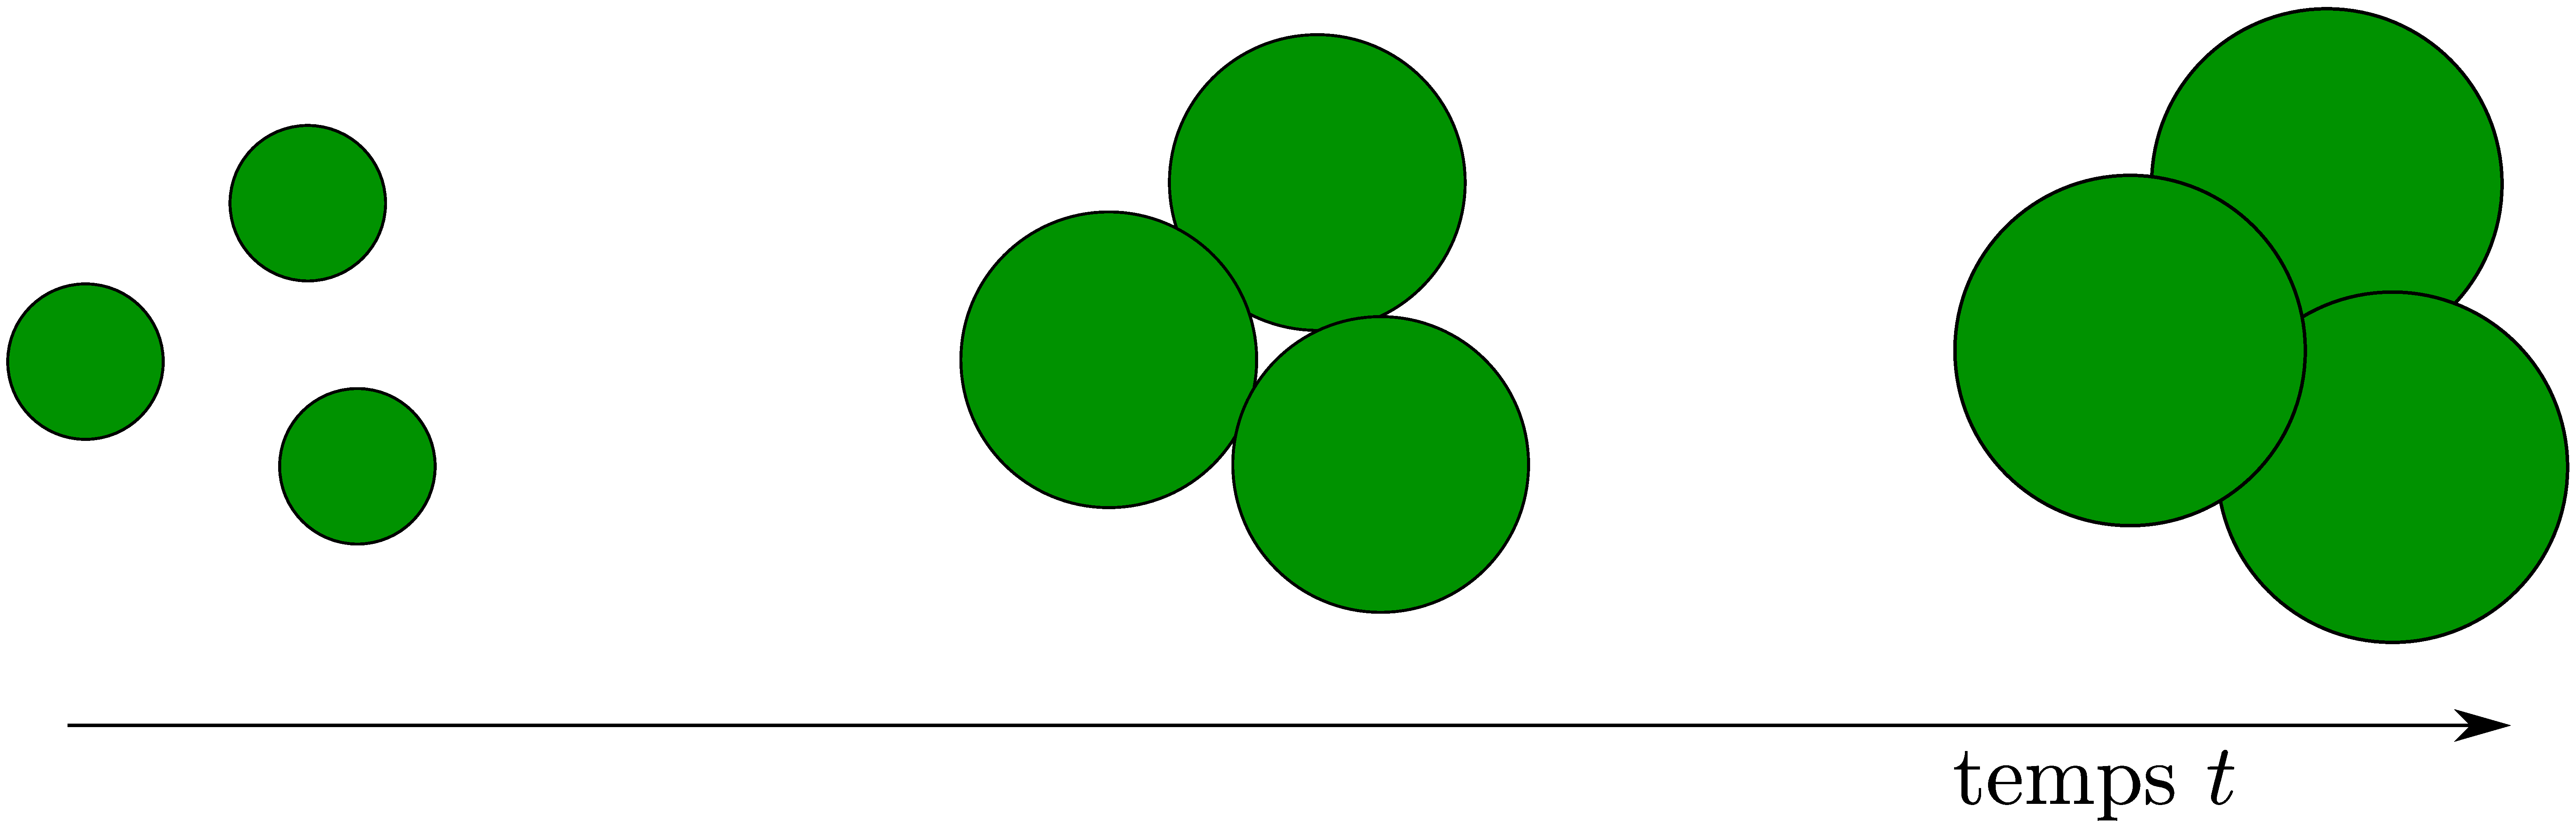
\includegraphics[width=12cm]{nenuphar.eps}
        \end{center}
	\vspace{-5mm}
	\caption{Évolution dans le temps de trois nénuphars.}\label{fig1}
\end{figure}

	Nous allons chercher à étudier l'évolution du nombre de \textit{trous} au cours du temps. On définira $u_n$ la suite indiquant le nombre de \textit{trous}. Pour bien définir cette suite, \begin{itemize}
\item elle devra avoir son premier et dernier termes nuls,
\item et deux termes consécutifs doivent toujours être différents.\\
\end{itemize}

	\subsection{Questions sur le modèle de \og croissance sans arrêt\fg}
\begin{enumerate}

	\item Supposons que sur un lac $L$ de forme arbitraire, nous avons un seul nénuphar. Quel est le temps $t_\mathrm{min}$ minimal nécessaire pour que le nénuphar recouvre tout le lac ? On supposera qu'il peut s'étendre sur la terre bordant le lac.

	\item Supposons maintenant que nous avons $2$ nénuphars. Donner une borne supérieure de $t_\mathrm{min}$. Cette borne peut-elle être atteinte et, si oui, dans quelle configuration ?\\

\noindent Supposons maintenant que le lac $L$ est infiniment grand.\\

	\item Quel est le nombre minimal de nénuphars pour qu'un \textit{trou} puisse se former ? Sous quelle condition géométrique cela peut il se produire (penser au centre du cercle circonscrit à un triangle) ? Formuler cette condition mathématiquement.

	\item Étant donnée la suite $u_n = \{ 0,1,3,0\}$, quel est le nombre minimal de nénuphars initialement présents sur le lac pour que cette séquence soit réalisable ? Donner une configuration initiale conduisant à cette suite. Mêmes questions pour la suite $u_n = \{ 0,1,3,0,1,0\}$.

	\item Si on considère $N$ nénuphars sur le lac, quelles sont toutes les suites $u_n$ possibles ?\\
\end{enumerate}

	\subsection{Croissance de génération en génération} Considérons un nouveau modèle. Nous allons maintenant supposer que lorsque deux nénuphars se rencontrent, ils reviennent alors à leurs positions initiales (i.e. comme à $t=0$). De plus, il apparaît au point de contact un nouveau nénuphar. Si deux rencontres ont lieu simultanément, on considèrera que deux nénuphars sont créés.\\

	On introduit la suite $v_n$ indiquant le nombre de nénuphars après la création du (ou des) $n$èmes individus (si plusieurs sont créés simultanément).\\

	\subsection{Questions sur le modèle \og croissance de génération en génération\fg}

\begin{enumerate}
	\item Considérons pour commencer une population de deux nénuphars à $t=0$. Comment va évoluer cette population au cours du temps ? Donner la suite $v_n$. Quelle figure observera-t-on avec les centres des nénuphars quand $t \rightarrow +\infty$ ?

	\item Poussons l'étude plus loin et considérons cette fois trois nénuphars initialement présents. Que se passe-t-il s'ils sont alignés ? S'ils ne sont pas alignés, délimiter une zone dans laquelle la population de nénuphars sera restreinte. Généraliser au cas de $N$ nénuphars.\\
\end{enumerate}



\section{Modélisation et extensions}

	Le but de cette partie sera à la fois de simuler l'évolution des nénuphars au cours du temps et d'approfondir notre étude à l'aide de l'outil numérique. On s'appuiera pour cela sur le logiciel Sage. Nous proposons ici quelques pistes d'étude que vous pouvez compléter avec de nouvelles si vous le souhaitez.

\subsection{Fabriquons des trous}

Dans cette section, on s'intéresse au modèle \og croissance sans arrêt\fg.

	\begin{enumerate}
		\item Étant donnée une configuration initiale de $N$ nénuphars sur un lac (modélisé par tout le plan), écrire un programme permettant d'afficher à un instant $t$ les nénuphars. Créer à partir de ce programme une animation en temps permettant de voir les nénuphars grandir.

        \item À l'aide de votre modèle, reproduisez les suites de \textit{trous} étudiées dans la première partie.

        \item Étant donnée une suite $u_n$, proposez un algorithme permettant de trouver une configuration initiale conduisant à cette suite.

	\end{enumerate}

\subsection{Cherchons les trous}

Il est beaucoup plus difficile de compter les trous que de les créer. Dans cette section, nous vous invitons à réfléchir à la question globale : \textbf{combien de trous possède une configuration quelconque à un temps donné ?}

\begin{enumerate}

\item Tout d'abord, on cherche à savoir si deux nénuphars sont en contact, écrivez cette fonction.

\item Écrivez une fonction qui vous donne les \textit{composantes connexes} de votre configuration, c'est-à-dire, les ensembles de nénuphars qui se touche entre eux. Créez un animation qui permet d'observer la croissance des nénuphars en mettant en évidence ces composantes grâce à des couleurs différentes.

\item Explorez la question principale. Une piste est d'utiliser l'objet \texttt{Graph} de Sage en construisant le graphe de la configuration.

\end{enumerate}

\subsection{Étude du modèle \og croissance de génération en génération\fg}
\begin{enumerate}
	\item Étant donnée un configuration initiale de $N$ nénuphars, écrire un programme permettant d'afficher au cours du temps la position des centres des nénuphars (marqués par exemple par un point).
	\item Faire le tracé de la suite $v_n$ à l'aide du simulateur précédent.
	\item Considérons que le lac n'est plus infini et que lorsqu'un nénuphar touche son bord, il disparaît. Écrire un programme permettant de simuler l'évolution d'une population de nénuphars au cours du temps. Tester une situation avec une île dans le lac.
\end{enumerate}


\subsection{Autres pistes !}
\begin{enumerate}
	\item Essayer de prendre un autre modèle de croissance des nénuphars, par exemple $R(t) = R_\mathrm{max} (1- e^{-t})$ avec $R_\mathrm{max}>0$. Dans ce modèle, les nénuphars ne grandissent pas indéfiniment.
	\item Prendre en compte un temps de vie des nénuphars.
	\item Changer la forme des nénuphars.
\end{enumerate}

\vspace{2cm}
\footnotesize{Image : Nénuphar géant, \url{https://commons.wikimedia.org/wiki/File:Nenuphar_geant.jpg}}

\end{document}